% -----------------------------------------------------------------------------
% The MIT License (MIT)
%
% Copyright (c) 2015 Pejman Ghorbanzade
%
% Permission is hereby granted, free of charge, to any person obtaining a copy
% of this software and associated documentation files (the "Software"), to deal
% in the Software without restriction, including without limitation the rights
% to use, copy, modify, merge, publish, distribute, sublicense, and/or sell
% copies of the Software, and to permit persons to whom the Software is
% furnished to do so, subject to the following conditions:
%
% The above copyright notice and this permission notice shall be included in
% all copies or substantial portions of the Software.
%
% THE SOFTWARE IS PROVIDED "AS IS", WITHOUT WARRANTY OF ANY KIND, EXPRESS OR
% IMPLIED, INCLUDING BUT NOT LIMITED TO THE WARRANTIES OF MERCHANTABILITY,
% FITNESS FOR A PARTICULAR PURPOSE AND NONINFRINGEMENT. IN NO EVENT SHALL THE
% AUTHORS OR COPYRIGHT HOLDERS BE LIABLE FOR ANY CLAIM, DAMAGES OR OTHER
% LIABILITY, WHETHER IN AN ACTION OF CONTRACT, TORT OR OTHERWISE, ARISING FROM,
% OUT OF OR IN CONNECTION WITH THE SOFTWARE OR THE USE OR OTHER DEALINGS IN
% THE SOFTWARE.
% -----------------------------------------------------------------------------

\section*{Question 1}
Back to Dalton Brothers! Develop a simple class \texttt{Brother.java} and its data memebrs and methods as you think best fits this program. Neglecting their original heights, write a program \texttt{Daltons3.java} that uses the \texttt{Brother.java} class to sort Joe, William, Jack and Averell after getting their heights from the user. The program should output names of the brothers in ascending order of their heights as specified.

\begin{figure}[H]\centering
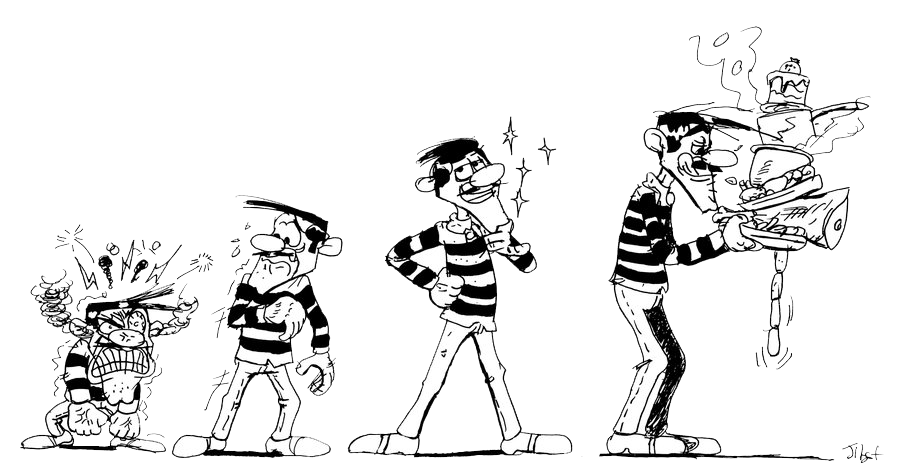
\includegraphics{\topDirectory/template/images/daltons.png}
\end{figure}

\subsection*{Solution}

\begin{enumerate}
\item Class \texttt{Brother.java}

\lstset{language=java,tabsize=2}
\begin{lstlisting}
public class Brother {
	public double height;
	public String name;
	public Brother(String hisName, double hisHeight) {
		height = hisHeight;
		name = hisName;
	}
	public Brother() {
	}
	public double getHeight() {
		return height;
	}
	public void setHeight(double height) {
		this.height = height;
	}
	public String getName() {
		return name;
	}
	public void setName(String name) {
		this.name = name;
	}
}
\end{lstlisting}

\item Class \texttt{DaltonsSort.java}
\lstset{language=java,tabsize=2}
\begin{lstlisting}
import java.util.Scanner;
public class DaltonsSort {
	public static void main(String[] args) {
		Scanner input = new Scanner(System.in);
		// Let's start with what we know: Names of brothers.
		String[] broNames = {"Joe", "William", "Jack", "Averell"};
		// Now that we can treat these brothers as humans (objects) not just variables,
		// Let's declare an array of objects and put all brothers in it.
		Brother[] bros = new Brother[broNames.length];
		// Now we can give identity to each brother by setting its name
		for (int i = 0; i < bros.length; i++){
			System.out.print("What is the height of " + broNames[i] + "? ");
			int height = input.nextInt();
			bros[i] = new Brother(broNames[i], height);
		}
		// So far, we have four brothers with different names and different heights
		// Let's ask user the sorting order
		System.out.print("In which order do you want to sort the Daltons [ASC, DESC]? ");
		String orderName = input.next();
		boolean orderAsc = orderName.equals("ASC") ? true : false;
		// Now we have all we want. Let's close the Scanner object then.
		input.close();
		// Time for sorting.
		for (int j = 0; j < bros.length; j++) {
			int minIndex = j;
			double min = Double.MAX_VALUE;
			for (int i = j; i < bros.length; i++) {
				if (bros[i].height < min) {
					min = bros[i].height;
					minIndex = i;
				}
			}
			if (j != minIndex) {
				Brother temp = new Brother();
				temp = bros[j];
				bros[j] = bros[minIndex];
				bros[minIndex] = temp;
			}
		}
		// Print names
		for (int i = 0; i < bros.length; i++) {
			System.out.println(orderAsc ? bros[i].getName() : bros[bros.length-1-i].getName());
		}
	}
}
\end{lstlisting}
\end{enumerate}

\section*{Question 2}
A student recently found a scrap of paper in MBTA Red line train on which the following code was written. Without modifying the code, develop a class \texttt{Elevator.java} to be used by this program.
\lstset{language=java,tabsize=2}
\begin{lstlisting}
public class ElevatorTest {
	public static void main(String[] args) {
		Elevator.currentLevel(); //outputs current floor
		Elevator.go(2); //moves the elevator two floors up
		Elevator.currentLevel();
	}
}
\end{lstlisting}

\subsection*{Solution}

Class \texttt{Elevator.java}
\lstset{language=java}
\begin{lstlisting}
public class Elevator {
	private static int floor;
	private final static int limitUp = 10;
	private final static int limitDown = -2;
	private Elevator() { floor = 0; }
	protected static void go(int level) {
		int dest = floor + level;
		if (dest <= limitUp && dest >= limitDown) {
			floor += level;
		}
		else {
			System.out.println("Impossible!");
		}
	}
	protected static void currentLevel() {
		System.out.println("Elevator is at floor "+floor);
	}
}
\end{lstlisting}

\section*{Question 3}

Objective is to simulate a circle-shaped pond with 100 meters radius, in which there are initially 100 salmons and one shark. As sharks and salmons know swimming, they continually wander around the pond. It's all about survival! To avoid starving to death, the shark must eat. To avoid extinction, salmons reproduce. Contrary to what it seems however, the shark has a very poor fate. If it doesn't eat for too long it will sadly die. If it manages to eat all the salmons and there are no more to eat, it won't be able to escape his destiny either. It's not about survival then. It's all about time!
\begin{figure}[H]\centering

\includegraphics[width=8cm,height=5cm]{\topDirectory/template/images/pond.png}
\end{figure}

Write a program \texttt{Simulation.java} that determines how many days the shark will live. Develop classes \texttt{Fish.java}, \texttt{Salmon.java}, \texttt{Shark.java} and \texttt{Pond.java} with their class members as you think best fits this program. Use the following assumptions.
\begin{itemize}[itemsep=1mm] \parskip=0pt \parsep=0pt
\item[] Fish are initially positioned randomly in the pond.
\item[] Fish move randomly in the pond.
\item[] Salmons move 10 meter per hour.
\item[] Salmons reproduce every day.
\item[] Salmons don't age and don't need to eat.
\item[] Salmons won't die unless they are eaten.
\item[] The shark moves 40 meters per hour in one direction.
\item[] The shark cannot eat while it's moving.
\item[] The shark is always hungry and never loses interest in eating.
\item[] The shark swallows all salmons within its 20 meters of proximity in a blink of an eye.
\item[] The shark dies if it does not eat in three days.
\item[] The shark is initially well fed.
\end{itemize}

\subsection*{Solution}

\begin{enumerate}
\item Class \texttt{Simulation.java}
\lstset{language=java, tabsize=2}
\begin{lstlisting}
import java.util.ArrayList;
public class Simulation {
	public static void main(String[] args) {
		initialize();
		while (shark.getHunger() < 3 * 24) {
			nextHour();
			eat();
			if (time % 24 == 0) {
				reproduce();
			}
			showStatistics();
		}
	}
	private static ArrayList<Salmon> salmons;
	private static Shark shark;
	private static int time = 0;
	// setup 100 salmons and 1 shark in Pond
	private static void initialize() {
		System.out.println("Initalizing Pond...");
		salmons = new ArrayList<Salmon>(101);
		for (int i = 0; i < 100; i++) {
			Salmon salmon = new Salmon();
			salmons.add(salmon);
		}
		shark = new Shark();
		System.out.println("Pond Initialized.");
	}
	// move all salmons and the shark
	private static void nextHour() {
		for (int i = 0; i < salmons.size(); i++) {
			salmons.get(i).move();
		}
		shark.move();
		time++;
	}
	// check if it's time to eat
	private static void eat() {
		double[] posShark = shark.getPosition();
		double[] posSalmon = new double[2];
		double dist;
		for (int i = salmons.size() - 1; i >= 0; i--) {
			posSalmon = salmons.get(i).getPosition();
			dist = Math.sqrt(Math.pow(posShark[0] - posSalmon[0], 2) + Math.pow(posShark[1] - posSalmon[1], 2));
			if (dist < shark.getRange()) {
				salmons.remove(i);
				shark.eat();
			}
		}
	}
	private static void reproduce() {
		int num = salmons.size();
		for (int i = 0; i < num; i++) {
			Salmon salmon = new Salmon(salmons.get(i).getPosition());
			salmons.add(salmon);
		}
	}
	private static void showStatistics() {
		System.out.printf("Time: %d\n", time);
		System.out.printf("Fish: %d\n", salmons.size());
		System.out.println();
	}
}
\end{lstlisting}
\item Class \texttt{Pond.java}
\lstset{language=java, tabsize=2}
\begin{lstlisting}
public class Pond {
	// Fields
	private static double radius = 100;
	// Instantiation should be forbidden
	private Pond() {}
	// Since radius of pond is fixed, setter for radius is not needed
	public static double getRadius() {
		return radius;
	}
}
\end{lstlisting}
\item Class \texttt{Fish.java}
\lstset{language=java, tabsize=2}
\begin{lstlisting}
public class Fish {
	// fields
	private static int numFish = 0;
	// attributes
	private double posRho;
	private double posAng;
	private double speed;
	// methods
	public void move() {
		double oldX = posRho * Math.cos(posAng);
		double oldY = posRho * Math.sin(posAng);
		while (true) {
			double theta = Math.random() * 2 * Math.PI;
			double newX = oldX + speed*Math.cos(theta);
			double newY = oldY + speed*Math.sin(theta);
			double newRho = Math.sqrt(Math.pow(newX,2) + Math.pow(newY,2));
			if (newRho < Pond.getRadius()) {
				posRho = newRho;
				posAng = Math.atan2(newY, newX);
				break;
			}
		}
	}
	// constructor
	public Fish() {
		posRho = Math.random() * Pond.getRadius();
		posAng = Math.random() * 2 * Math.PI;
		numFish++;
	}
	public Fish(double[] position) {
		posRho = Math.sqrt(Math.pow(position[0], 2) + Math.pow(position[1], 2));
		posAng = Math.atan2(position[1], position[0]);
		numFish++;
	}
	// getter and setter for position
	public void setSpeed(double speed) {
		this.speed = speed;
	}
	public static int getNumFish() {
		return numFish;
	}
	public double[] getPosition() {
		double[] position = new double[2];
		position[0] = posRho * Math.cos(posAng);
		position[1] = posRho * Math.sin(posAng);
		return position;
	}
}
\end{lstlisting}
\item Class \texttt{Salmon.java}
\lstset{language=java, tabsize=2}
\begin{lstlisting}
public class Salmon extends Fish {
	private static int numSalmons = 0;
	public Salmon() {
		super();
		setSpeed(10);
		numSalmons++;
	}
	public Salmon(double[] position) {
		super(position);
		setSpeed(10);
		numSalmons++;
	}
	public static int getNumSalmons() {
		return numSalmons;
	}
}
\end{lstlisting}
\item Class \texttt{Shark.java}
\lstset{language=java, tabsize=2}
\begin{lstlisting}
public class Shark extends Fish{
	private static int numSharks = 0;
	private int hunger = 0;
	private double range = 20;
	public Shark() {
		super();
		setSpeed(40);
		numSharks++;
	}
	public void move() {
		super.move();
		hunger++;
	}
	public static int getNumSharks() {
		return numSharks;
	}
	public int getHunger() {
		return hunger;
	}
	public void eat() {
		hunger = 0;
	}
	public double getRange() {
		return range;
	}
}
\end{lstlisting}
\end{enumerate}
